\documentclass{article}

\usepackage[utf8]{inputenc}
\usepackage[backend=biber, style=numeric]{biblatex}
\usepackage[dutch]{babel}
\usepackage{fancyhdr}
\usepackage{graphicx}
\usepackage{float}
\usepackage{booktabs}
\usepackage{subcaption}


\pagestyle{fancy}
\fancyhf{}
\rhead{ Scaling }
\lhead{Meetrapport}
\rfoot{Pagina \thepage }

\begin{document}
\author{Dimitry Volker}
\makeatletter
    \begin{titlepage}
        \begin{center}
            {\huge \bfseries  \@title }\\[2ex] 
            {\LARGE Meetrapport, Snelheid - Scaling}\\[10ex]
            
            {\large \@author - 1661152}\\
            {\large Jasper van Hulst - 1660498}\\[5ex]
            {\large \@date}
            
            \vskip4em%
        \end{center}
    \end{titlepage}
\makeatother
\thispagestyle{empty}

\clearpage

\renewcommand{\contentsname}{Inhoudsopgave}
\tableofcontents

\clearpage

\section{Doel}
Het schalen van een afbeelding is op diverse manieren voor elkaar te krijgen. Er bestaan 3 algoritmes die veel op elkaar lijken "Nearest-neighbour Interpolation", "Bilinear Interpolation" en "Bicubic Interpolation". Als er een situatie zich voordoet dat het verkleinen of het vergroten nodig is voor duidelijkheid, is het goed om te weten welk algoritme je moet gebruiken. 

\begin{center}
    "Welk algoritme schaalt met de beste kwaliteit dat met het oog te zien is?".   
\end{center}

Om deze vraag te beantwoorden zal er gekeken worden naar de kwaliteit van de geschaalde afbeeldingen.

\section{Hypothese}

Het lijkt ons aannemelijk dat "Bicubic Interpolatie" het beste zal functioneren. Door een groter veld te pakken (16 bij 16 pixels) zullen de overgangen zachter zijn en blijven details meer intact. Overigens denken wij dat Nearest-neighbour de slechtste kwaliteit zal hebben. 

\section{Onderzoeksmethode}
Om een goed beeld te krijgen van de kwaliteit zetten we de geschaalde afbeeldingen naast elkaar. Zo is het mogelijk om de kwaliteit te vergelijken.

\begin{figure}[H]
    \centering
    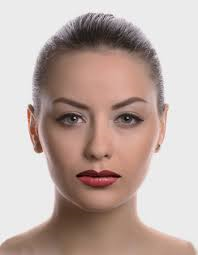
\includegraphics{assets/female-3.png}
    \caption{Orginele afbeelding}
    \label{fig:my_label}
\end{figure}

\section{Resultaten}



\subsection{Schalingsfactor 0.5}

\begin{figure}[H]
\centering
    \begin{subfigure}{.5\textwidth}
      \centering
      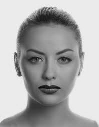
\includegraphics[]{assets/Bicubic_Female_05.png}
      \caption{Bicubic, scalingfactor: 0.5}
      \label{fig:sub1}
    \end{subfigure}%
    \begin{subfigure}{.5\textwidth}
      \centering
      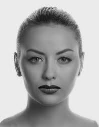
\includegraphics[]{assets/Bilinear_Female_05.png}
      \caption{Bilinear, scalingfactor: 0.5}
      \label{fig:sub2}
    \end{subfigure}
    \begin{subfigure}{.5\textwidth}
      \centering
      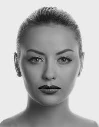
\includegraphics[]{assets/Nearest_Female_05.png}
      \caption{Nearest-Neighbour, scalingfactor: 0.5}
      \label{fig:sub3}
    \end{subfigure}
    \caption{Schalen met factor 0.5}
    \label{fig:test}
\end{figure}

\clearpage
\subsection{Schalingsfactor 0.75}

\begin{figure}[H]
\centering
    \begin{subfigure}{.5\textwidth}
      \centering
      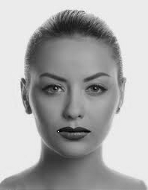
\includegraphics[]{assets/Bicubic_Female_075.png}
      \caption{Bicubic, scalingfactor: 0.75}
      \label{fig:sub1}
    \end{subfigure}%
    \begin{subfigure}{.5\textwidth}
      \centering
      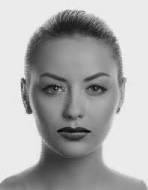
\includegraphics[]{assets/Bilinear_Female_075.png}
      \caption{Bilinear, scalingfactor: 0.75}
      \label{fig:sub2}
    \end{subfigure}
    \begin{subfigure}{.5\textwidth}
      \centering
      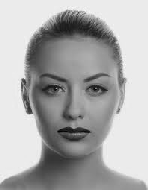
\includegraphics[]{assets/Nearest_Female_075.png}
      \caption{Nearest-Neighbour, scalingfactor: 0.75}
      \label{fig:sub3}
    \end{subfigure}
    \caption{Schalen met factor 0.75}
    \label{fig:test}
\end{figure}

\clearpage
\subsection{Schalingsfactor 1.25}

   \begin{figure}[H]
      \centering
      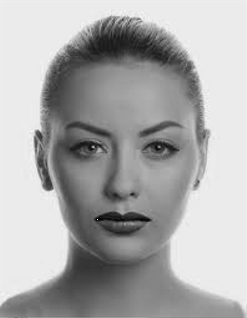
\includegraphics[]{assets/Bicubic_Female_125.png}
      \caption{Bicubic, scalingfactor: 1.25}
      \label{fig:sub1}
    \end{figure}%
    \begin{figure}[H]
      \centering
      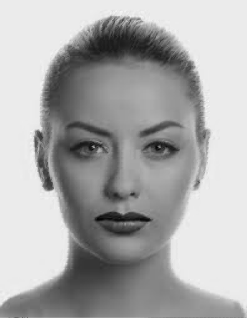
\includegraphics[]{assets/Bilinear_Female_125.png}
      \caption{Bilinear, scalingfactor: 1.25}
      \label{fig:sub2}
    \end{figure}
    \begin{figure}[H]
      \centering
      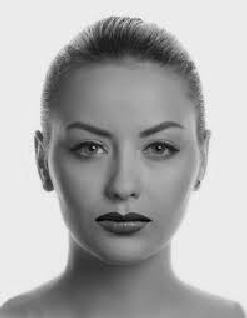
\includegraphics[]{assets/Nearest_Female_125.png}
      \caption{Nearest-Neighbour, scalingfactor: 1.25}
      \label{fig:sub3}
    \end{figure}
    
\clearpage
\subsection{Schalingsfactor 1.5}

   \begin{figure}[H]
      \centering
      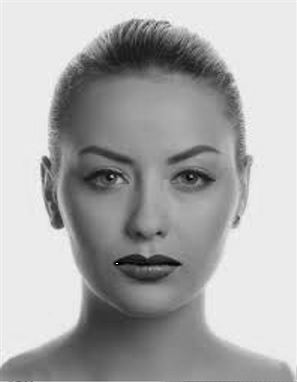
\includegraphics[]{assets/Bicubic_Female_15.png}
      \caption{Bicubic, scalingfactor: 1.5}
      \label{fig:sub1}
    \end{figure}%
    \begin{figure}[H]
      \centering
      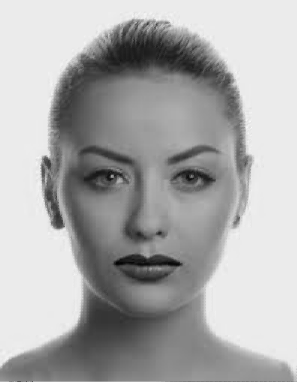
\includegraphics[]{assets/Bilinear_Female_15.png}
      \caption{Bilinear, scalingfactor: 1.5}
      \label{fig:sub2}
    \end{figure}
    \begin{figure}[H]
      \centering
      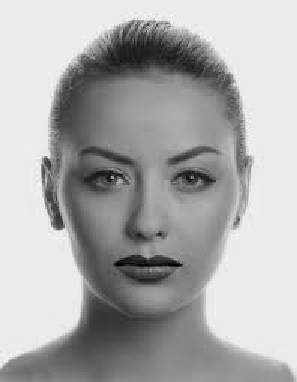
\includegraphics[]{assets/Nearest_Female_15.png}
      \caption{Nearest-Neighbour, scalingfactor: 1.5}
      \label{fig:sub3}
    \end{figure}
    
\section{Conclusie}
Het is duidelijk te zien dat "Bicubic Interpolation" meer details bewaart tijdens het schalen. Dit is vooral te zien aan het vergroten van een afbeelding. Wanneer de afbeelding wordt verkleind lijken Bicubic en Bilinear nagenoeg gelijk aan elkaar.
\end{document}